\documentclass[12pt,a4paper,oneside,english]{book}

\usepackage{cite}


%\usepackage[latin1]{inputenc}

%\usepackage[T1]{fontenc}
\usepackage[english]{babel}
\usepackage{amsmath}
\usepackage{amsfonts}
\usepackage{amssymb}
\usepackage{graphicx}
\usepackage{subfig}
\usepackage{fancyhdr}
\usepackage{appendix}
\usepackage{hyphenat}
\usepackage{pdfpages}
\usepackage{svg}

%\usepackage{tocloft} % For TOC customization ( table of contents )
\usepackage{array,multirow,makecell}
\newcolumntype{C}[1]{>{\arraybackslash}p{#1}}

\usepackage{enumitem}
\setlist{leftmargin=*,itemsep=0pt}

\usepackage{centernot}
\usepackage[linesnumbered,ruled,vlined,english,onelanguage]{algorithm2e}

\usepackage{quotchap}
\makeatletter
\renewcommand{\@makechapterhead}[1]{
 \chapterheadstartvskip
 {\size@chapter{\sectfont\raggedright
 {\chapnumfont
 \ifnum \c@secnumdepth >\m@ne
 \if@mainmatter\thechapter %frontmatter for roman numerals
 \fi\fi
 \par\nobreak}
 {\raggedright\advance\leftmargin10em\interlinepenalty\@M #1\par}}
 \nobreak\chapterheadendvskip}}
\makeatother
\renewcommand*{\chapterheadendvskip}{\vspace{2cm}}
%\renewcommand{\thechapter}{\Roman{chapter}} % Set chapter numbering to Roman numerals


\usepackage{geometry}
\geometry{hmargin=2cm,vmargin=2cm}

\pagestyle{fancyplain}
\lhead{\fancyplain{}{\nouppercase{\textit{\leftmark}}}}
\chead{\fancyplain{}{}}
\rhead{\fancyplain{}{}}
\lfoot{\fancyplain{}{}}
\cfoot{\fancyplain{}{}}
\rfoot{\fancyplain{\thepage}{\thepage}}
\renewcommand{\headrulewidth}{1pt}
\renewcommand{\footrulewidth}{1pt}

\renewcommand{\thesection}{\Roman{section}} % Set section numbering to Roman numerals % previously \arabic{section}

\usepackage{titlesec}
\titleformat{\paragraph}{\fontsize{11}{10}\bfseries}{\theparagraph}{1em}{}
\titlespacing*{\paragraph}{0pt}{10pt plus 2pt minus 0pt}{0pt plus 2pt minus 0pt}

\setcounter{secnumdepth}{4}
\setcounter{tocdepth}{4}

%%%%%
\usepackage{listings}
\usepackage{xcolor} % Required for colors

% Define a custom style for JSON
\lstdefinestyle{jsonstyle-compact}{
    language=Java, % listings doesn't have a JSON language, but Java is close enough
    basicstyle=\footnotesize\ttfamily, % Use a smaller font
    keywordstyle=\color{blue},
    stringstyle=\color{black},
    commentstyle=\color{green},
    morestring=[b]",
    showstringspaces=false,
    breaklines=true,
    frame=none, % Remove the frame/rectangle
    backgroundcolor= \color{gray!5} %{gray!10}
}
%%%


\usepackage{array}
\usepackage{multirow}
%\addto\captionsfrench{\def\tablename{\textsc{Tableau}}}

%\DefineBibliographyStrings{french}{urlseen = {},}

\setlength{\parskip}{0pt}%was 8 : space between paragraphs
\setlength{\parindent}{1.5em}%was 1.5 : indentation of paragraphs

\usepackage{setspace}

\usepackage{url}

\usepackage{hyperref}
% Comment before printing to remove links' colors
\definecolor{darkblue}{rgb}{0.0, 0.0, 0.5}
\hypersetup{
 colorlinks,
 linktocpage=true,
 linkcolor={darkblue},
 citecolor={darkblue},
 urlcolor={blue}}

\sloppy

\author{You}
\title{Internship Report}

\begin{document}
\pagenumbering{gobble}
\includepdf[pages=-]{FrontPage.pdf}
\chapter*{Acknowledgments}

\frontmatter %here yothhrou les num des pages en bas 
\chapter*{Abstract}
\normalsize{Write your abstract here.

\medskip
{\noindent \textbf{Keywords: ..., ... .} }

\spacing{1}
\tableofcontents{}
\newpage 
\listoffigures
\newpage 
\listoftables
\newpage
\spacing{1.4}
\chapter*{List of acronyms}
%\addcontentsline{toc}{chapter}{Liste des acronymes}
\markboth{List of acronyms}{}%abbrev
\begin{itemize}
\item \textbf{AI} Artificial Intelligence
\item \textbf{ML} Machine Learning
\item \textbf{API} Application Programming Interface
\item \textbf{ASR} Automatic Speech Recognition
\item \textbf{SER} Speech Emotion Recognition
\item  \textbf{NLP} Natural Language Processing
\item \textbf{DBSCAN} Density-Based Spatial Clustering of Applications with Noise
\item \textbf{GIS} Geographical Information System
\item \textbf{GPS} Global Positioning System
\item \textbf{BERT} Bidirectional Encoder Representations from Transformers
\end{itemize}

\frontmatter %here yothhrou les num des pages fl contnent
%\frontmatter  %to have roman page numbering in the beginning
%\mtcaddchapter[Introduction g�n�rale]

\chapter*{Introduction}
\addcontentsline{toc}{chapter}{Introduction}
\markboth{Introduction}{}

\chapter{Company Presentation} % we should metion that there are a lot of spacing between title of chapter and sctions

\label{ch:1er}
\section{Overview}
Founded in 2020, and located in both Meudon la forêt , Meudonn France and tunis, Tunisia, 
Hydatis is dedicated to helping early-stage companies leverage the latest data intelligence and digital technologies to solve real-world challenges, becoming, since then, a leading technology startup studio with a proven track record.
\begin{figure}[h!] % placement options: h=here, t=top, b=bottom, p=page
    \centering
    
\includegraphics[width=0.2\textwidth]{images/hydatiss.png}
    \caption{Logo of Hydatis}
    \label{fig:hydatis}
\end{figure}

Hydatis specializes in AI, machine learning, blockchain, big data Analysis and more. Hydatis's team of technology experts is dedicated to building scalable and sustainable businesses, with a focus on creativity, strategy, and technology alongside with a vast network of partners and investors and a strong reputation in the technology industry.
\begin{figure}[h!] % placement options: h=here, t=top, b=bottom, p=page
    \centering
    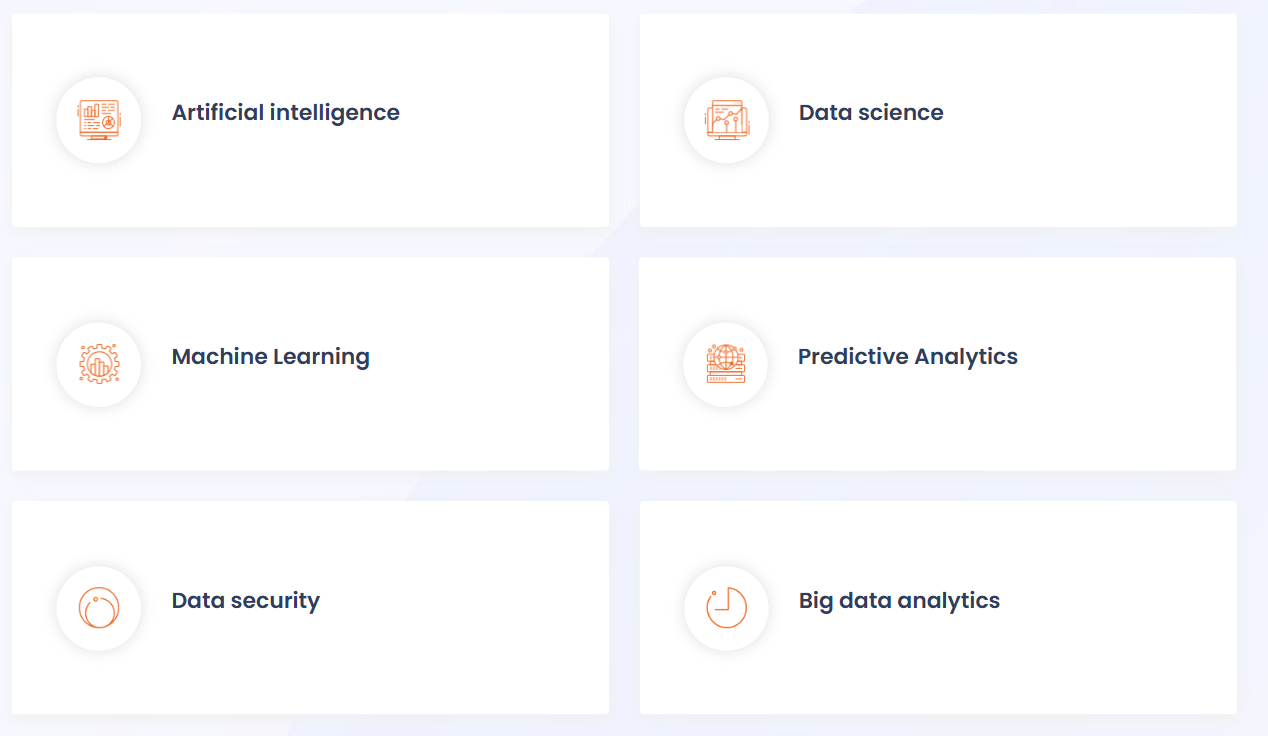
\includegraphics[width=0.699\textwidth]{images/Expertise_hydatis.png}
    \caption{Hydatis' Areas of Expertise}
    \label{fig:Expertise_hydatis}
\end{figure}

\section{Sectors of Activities}%and services offered
Hydatis is a product-focused Tech venture studio offering a range of services tailored to the unique needs of each startup, including:
 business planning, product development, marketing, and fundraising. 
%With their expertise in data analytics, machine learning, and other advanced technologies, 
Leveraging technology and entrepreneurship, they help clients turn data into actionable insights that drive business success.
%help businesses make big decisions about their future by making tangible versions of tomorrow.
\subsection{Services offered}
\begin{itemize}
    \item \textbf {Software development Services}
    \item \textbf{CTO as a service}
    \item \textbf{IT Consulting}
    \item \textbf{Devops Consulting}
    \item \textbf{and a lot more...}
\end{itemize}
\begin{figure}[h!]
    \centering
    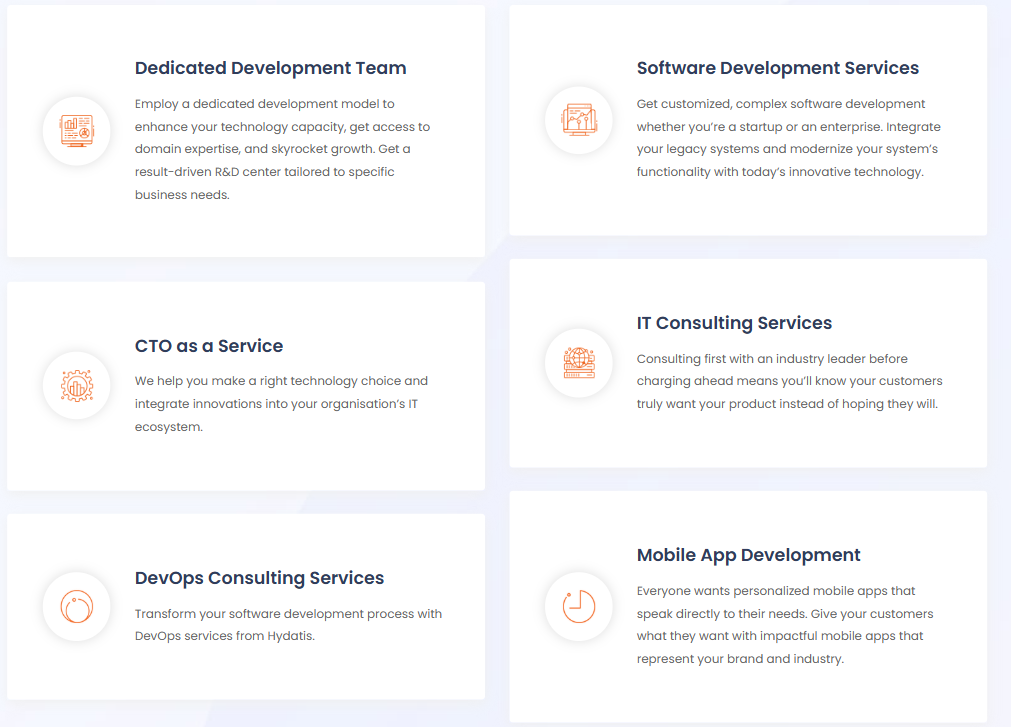
\includegraphics[width=0.9\textwidth]{images/services_hydatis.png}
    \caption{Hydatis' Services}
    \label{fig:Services_hydatis}
\end{figure}

\section{Organizational structure and Human Capital} % eithr this part will be deleted or the susection in the activities section will be modified and either discard items or having an individual subsection
Hydatis with a flat organizational structure that reflects its startup studio roots, led by  expertised directors who drive strategy and innovation alongside a talented crew of entrepreneurs and technologists, business strategists and network coordinators.

From AI specialists shaping cutting-edge products to strategists securing partnerships, and sicne its launch in 2020, these folks, with their varied backgrounds, suceeded to make Hydatis a powerhouse in the startup ecosystem.


\chapter{Internship Context and Objectives}
\label{ch:2eme}
\section{Problem Statement and Motivation} %Why
Crime is a major social problem in Tunisia, threatening public safety and disrupting the economy,ranging from theft to harassment, often leaving individuals vulnerable, especially at night or in isolated spots.
 
Traditional safety solutions such as manual reporting or basic wearable alarms have served as a foundational step in personal security. However they %struggle
suffer from critical limitations: 
The binary nature of a simple button press is usually unsufficient to distinguish between 
a genuine, life-threatening emergency,a false alarm, or a low-priority situation.
Additionally, the lack of contextual awarness results in inaccurate alerts and overwhelming emergency services with false positives. %Inaccuracy and Context Deficiency:
Giving the limited resources of emergency services (police, paramedics), false alarms divert critical attention away from genuine crises, incurring unnecessary costs and potentially delaying responses to real incidents. %Resource Depletion:


%The binary nature of a simple button press: unsufficient to distinguish between 
%a genuine, life-threatening emergency,a false alarm, or a low-priority situation. This leads to an unacceptably 
%high rate of false positives.

%  This gap hits home for Hydatis, the motivation behind this work is clear: we need to move beyond simple, reactive triggers
% and build smarter, faster ways to protect people by qualifying alerts with precision.
\subsection{Market Context and Existing Solutions}

Several commercial solutions exist in the personal safety market, including panic button apps like 
bSafe, location-sharing platforms like Life360, and wearable devices such as personal alarms. However,
 these solutions typically operate independently and lack the intelligent analysis needed to 
 differentiate between genuine emergencies and false alarms and ensure fast response to threats. 
 %, leading to the limitations described above.
Therefore, there is a clear need for an intelligent safety system that can analyze multiple data 
streams—location, audio, and behavioral patterns—to provide accurate, context-aware emergency 
detection while minimizing false positives.

%In State of the Art, you can include:
%Existing products (apps, devices, services → e.g., SOS apps, smartwatches with panic buttons, crime reporting platforms).
%Research/technical approaches (papers on anomaly detection, crime prediction models, wearable safety devices).
%Limitations of these (false positives, lack of contextual awareness, poor adoption, battery issues, limited reach, etc.).

%Detailed technical comparisons
%Algorithm discussions
%Academic literature reviews
%In-depth analysis of existing methods

%todo: reduce space in the footer ( especially see this page!)
%todo: and fama paget fihom khatt fl footer o whayed lee

\section{Description}% or scope : the "What." and "how" A high-level overview of the solution.

This project involves designing an AI-powered module for a Smart wearable Solution, aimed at enhancing personal safety through automated incident detection during my Summer internship at Hydatis.
The module integrates four key data streams: 
\begin{itemize}
    \item \textbf{Geospatial Analysis:} geospatial data derived from Tunisian crime datasets to identify high-risk areas.
    \item \textbf{Vocal Signal Processing:}  real-time vocal analysis to detect distress signals or key words such as calls for help.
    \item \textbf{Behavioral Profiling:} behavioral patterns to flag anomalies in user activitythat may indicate danger.
    \item \textbf{Decision Engine:} later, these components are fused into a cohesive system that processes and combines 
insights from each stream, offering a foundation for reliable alert qualification.
\end{itemize}
Though, detailed implementation will be explored in later sections.


\section{Core Mission, Objectives and Expected Results}

\subsection{Core Mission}
My core mission in this project is to develop an intelligent, multi-modal safety system that integrates  geospatial analysis, vocal processing, and behavioral profiling to transform personal security and  provide accurate , context-aware emergency detection that minimizes false alarms while ensuring genuine immediate attention to genuine threats  .

\subsection{Main Objectives}

\textbf{Technical Objectives:}
\begin{itemize}
    \item Achieve a minimum of 80\% accuracy in alert qualification.
    \item Minimize false positive rates. 
    \item Enable real-time processing  with response times under 5 seconds.
    \item Design a robust system capable of handling diverse scenarios and user behaviors.
\end{itemize}

\textbf{Implementation Objectives:}
\begin{itemize}

\item Process a Tunisian crime dataset for geospatial risk assessment.
\item Train a vocal ASR model adapted to Tunisian dialects for distress-related risk detection.
\item Prepare a vocal pipeline to analyse vocal patterns including: tone, rythm, and pitch.
\item Design a comprehensive database of processed behavioral patterns for every user.
   \item Integrate three distinct AI modules (geospatial, vocal, behavioral) into a cohesive system.
    \item Develop a proof-of-concept API for periodic risk assessment and scoring alerts.
    \item Ensure system scalability for potential deployment beyond Tunisia.
\end{itemize}

\subsection{Expected Results}
\begin{itemize}
\item A cleaned and structured Tunisian crime dataset inferred to geospatial risk analysis.
\item An ASR model integrated for vocal analysis in tunisian Arabic. %supporting real-time distress detection.
\item A vocal pipeline capable of analysing vocal patterns of stress and/or fear.
\item ML models designed for inferring  users behaviors.
\item A proof-of-concept multi-modal scoring system with sub-5-second responses.
\item APIs developed for periodic risk assessment and potential integration into a mobile or web interface.
\end{itemize}


\section{Internship timeline }% or planning %professionalism and project management skills.%%%%%often a Gantt chart)
%Timeline = just dates and deadlines
%Planning = timeline + methodology + resources + milestones

This project is structured over my two-month internship period at Hydatis, devided into:
\begin{itemize}
    \item \textbf{Weeks 1-2:} Initial research, dataset acquisition, and preprocessing.
    \item \textbf{Weeks 3-4:} Development of the geospatial analysis module and initial vocal processing pipeline.
    \item \textbf{Weeks 5-6:} Behavioral profiling model development and integration of the three AI modules.
    \item \textbf{Weeks 7-8:} Final system integration, testing, optimization, and documentation.
\end{itemize}

%todo: label the sections and subsections
%todo: diagramme de gantt!!!!

\chapter{Theoritical Foundations and State of the Art}
\label{ch:3eme}

% normalement we should put here:  State of the Art and Market Solutions section
% or subsection in the motivation and problem statement section: Existing Solutions and Limitations”
\section*{Introdunction}
This chapter presents the theoretical foundations underlying the proposed multi-modal safety system, which integrates three distinct yet complementary technologies:

First, the principles of geospatial analysis for risk prediction will be examined. 
Second, the field of vocal signal processing for distress detection will be explored, detailing the methods used to identify audible signs of an emergency from a user's speech. 
Finally, the concepts of machine learning applied on behavioral anomaly detection will be discussed, explaining the detection of anomalies based on personal routines.
\\This review justifies the technical choices made in the subsequent implementation chapter.
%establishes the scientific basis for
\section{Geospatical Analysis for Risk Prediction}
\label{sec:geospatial_theory}

Geospatial analysis integrates Geographical Information Systems (GIS) with advanced analytical techniques to identify crime hotspots, cluster incidents, and enable real-time risk assessment. This section explores hotspot forecasting, density-based clustering, and the evolution toward real-time systems, aligning with the need for intelligent personal safety solutions.

%This section establishes the theoretical foundations for location-based risk assessment module, which forms a core component 
%of the proposed multi-modal safety system.
%The analysis begins with crime hotspot theory and spatial clustering principles. Subsequently, density-based clustering algorithms, 
%particularly DBSCAN, are examined. Finally, the transition from static crime mapping to real-time risk assessment systems is explored.


\subsection{Crime Hotspot Forecasting and Spatial Analysis}


%Geospatial anomaly detection leverages Geographical Information Systems (GIS) to identify unusual patterns in spatial data, 
%a critical step in predicting crime hotspots. GIS integrates spatial datasets—such as crime locations, demographic details, 
%and environmental factors—into a unified framework for analysis [El-Fishawy et al., 2024]. 
%W ANTED TO PUT IT HERE

The foundational principle of crime hotspot analysis is that criminal activity is not randomly 
distributed, but rather concentrated in specific areas known as 'hotspots'
This involves analyzing geographic patterns where crime incidents cluster,
often influenced by factors like urban density or offender homogeneity \cite{chen2019exploring}. 
Hotspot theory posits that such clusters represent areas of elevated risk, necessitating targeted interventions  \cite{zhuang2017crime} .
With the ever-increasing ability of states and organizations to collect and store detailed data tracking crime occurrence, a significant amount of data with spatial and temporal information has been collected
In this context, these hotspots, defined as deviations from expected spatial-temporal behavior, can be treated as a form of spatial anomaly and can be detected using statistical and machine learning techniques, enabling the identification of high-risk areas.

\subsection{Density-Based Clustering for Spatial Data}%or for geographic data
\label{sec:dbscan_theory}
Crime data is inherently noisy and unevenly distributed, making it challenging to identify meaningful patterns using simple statistical methods. Clustering techniques are therefore employed to detect areas 
where incidents concentrate, which often correspond to crime hotspots.
%Spatial clustering is a process of grouping objects based on their spatial similarity. 

Among the available clustering algorithms, density-based methods such as DBSCAN \textbf{(Density-Based Spatial Clustering of Applications with Noise) } \cite{BIRANT2007208dbscan} are particularly effective for spatial data, a method well-suited for irregular,
 non-spherical patterns.
 \\
DBSCAN groups data points that are closely packed together and marks outliers as noise based on their density in the feature space.
Unlike other methods of clustering such as K-Means, it performs well in handling real-world data irregularities such as:
\begin{itemize}
    \item Arbitrary-Shaped Clusters: Clusters can take any shape not just circular or convex.
    \item Noise and Outliers: It effectively identifies and handles noise points without assigning them to any cluster.
\end{itemize}

\begin{figure}[h!] % placement options: h=here, t=top, b=bottom, p=page
    \centering
    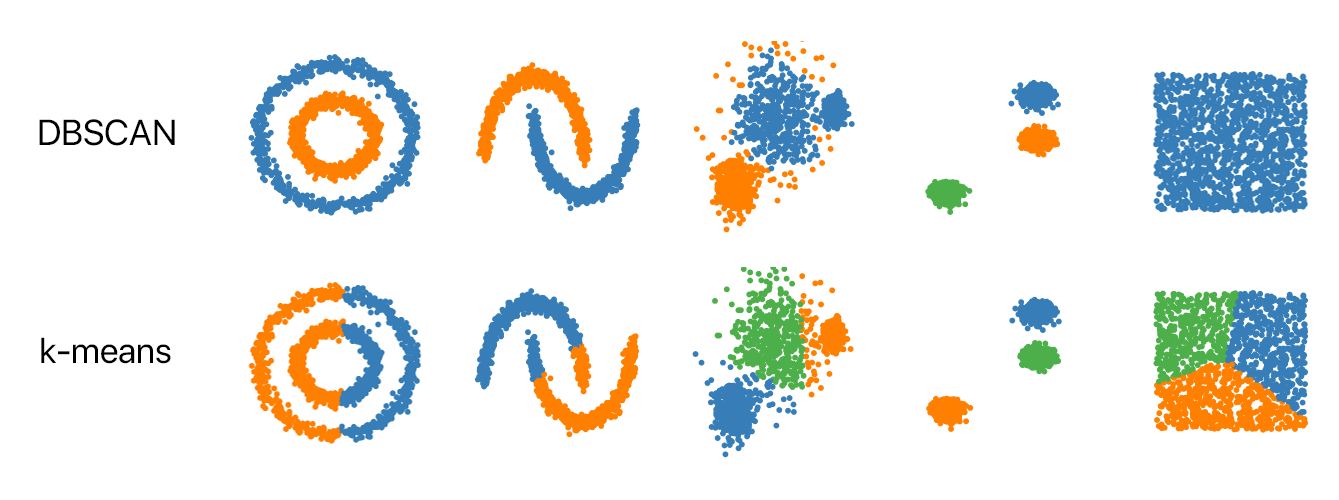
\includegraphics[width=0.5\textwidth]{images/dbscanVSkmeans.png}
    \captionsetup{width=0.6\textwidth}
    \caption{A comparison showing DBSCAN's ability to identify non-spherical clusters, in contrast to K-Means.}
    %\caption{DBSCAN Clustering Compared to K-Means: DBSCAN can identify clusters of arbitrary shapes and effectively handle noise, while K-Means tends to form spherical clusters and is sensitive to outliers.}
    \label{fig:dbscan_vs_kmeans}
\end{figure}

Key Parameters in DBSCAN:
\begin{itemize}
    \item eps ($\epsilon$): The maximum distance between two samples for one to be considered as in the neighborhood of the other.
    \item MinPts: This is the minimum number of points required within the eps radius to form a dense region. 
\end{itemize}
%1. eps: defines the radius of the neighborhood around a data point. Commonly determined with a k-distance graph Analysis. 
%Choosing the ips is Critical: If eps is too small most points will be classified as noise and if it is too large clusters may merge and the algorithm may fail to distinguish between them.
%2. MinPts: This is the minimum number of points required within the eps radius to form a dense region. 
%For most cases a minimum value of MinPts = 3 is recommended


These characteristics make DBSCAN exceptionally well-suited for analyzing real-world crime pattern.
This approach is validated by recent research: Chen et al. \cite{chen2019exploring} successfully utilized an extension of DBSCAN to detect crime hotspots from historical theft records %, validating its effectiveness in this domain

\subsection{Real-time Risk Assessment Systems}%or relevance to risk prediction
% Current approaches, GPS-based risk scoring, challenges in real-time implementation
Real-time geospatial risk assessment is the practical application of crime hotspot forecasting in operational safety systems.
While traditional approaches rely on static crime databases and predetermined risk zones, the challenge lies in integrating GPS-enabled systems to continuously process  spatial data  to calculate immidiate risk score.
\\This is the evolution from static hotspot analysis systems to active safety systems.






\section{Vocal Signal Processing for Distress Detection}
\label{vocal_processing_theory}
In real world emergencies, vocal cues such as tone, pitch, and specific keywords can provide critical 
insights into a person's state of distress. This section explores the theoretical foundations of vocal signal processing: 
Speech Emotion Recognition (SER) for emotional states detection %for detecting emotional states from audio signals, 
,Automatic Speech Recognition (ASR) for speech transcription% for transcribing spoken words 
and Natural Language Processing (NLP) for intent analysis. %for analyzing the transcribed text for intent and risk assessment.


\subsection{Speech Emotion Recognition (SER)}%emotion recognition from speech
\label{ser}
Speech contains important information beyond the words themselves, such as the speacker's emotion, pitch and tone.
Speech Emotion Recognition (SER) is the field of study focused on automatically identifying the emotional state of a speaker from their voice by analyzing acoustic and prosodic features—such as pitch, tone, and energy—to classify emotions like anger, happiness, or fear.
\\The process begins with feature extraction, a foundational concept, where meaningful data is derived from the raw audio signal, often using preprocessing  tools like \textbf{Librosa} \cite{librosa}.%todo cite it
\\Modern SER systems employ transformer-based architectures like \textbf{Wav2Vec 2.0} \cite{NEURIPS2020_92d1e1ebWav2Vec} 
which is a self-supervised model that demonstrates superior performance through pre-training on diverse audio data followed by task-specific fine-tuning.
\\For instance, research has shown that Wav2Vec 2.0 can reach an accuracy of 79.58\% on the IEMOCAP benchmark\cite{wang2022finetunedwav2vec20hubertbenchmark},% [Wang et al., 2022], %todo here we cite the paper fl okhrin we cite the offical documentation
validating its selection as a robust theoretical foundation for the distress detection module.


\subsection{Automatic Speech Recognition (ASR)}%speech-to-text conversion
\label{asr}
Automatic Speech Recognition (ASR) is the process of converting spoken language into written text, enabling machines to understand and process human speech.
The Progress in speech recognition has been energized by the development of unsupervised pre-training techniques exemplified by Wav2Vec 2.0 \cite{NEURIPS2020_92d1e1ebWav2Vec} (See \ref{ser}).  
This suggests that while unsupervised pre-training has improved the quality of audio encoders dramatically, the lack
of an equivalently high-quality pre-trained decoder, combined with a recommended protocol of dataset-specific fine
tuning, is a crucial weakness which limits their usefulness and robustness.  

For this, OpenAI implemented \textbf{Whipser}, \cite{pmlr-v139-radford21aWhisper} a Transformer-based model trained on a massive 680,000 hours of diverse audio, enabling it to perform robustly in a zero-shot setting without  
Reaserchers have also worked on a bench of versions of Whisper focusing on more epochs while adding, SpecAugment Stochastic Depth, or BPE Dropout, forming a family of Tiny, Medium, Large architectures\dots \cite{pmlr-v139-radford21aWhisper}

%Whisper models, which are trained on a broad and diverse distribution of audio and evaluated in a zero-shot setting,  
Whisper models could potentially match human behavior much better than existing systems.
To assert their efficiency, comparaisons between  Whisper models with both human performance
 and standard fine-tuned ML models were done. Whisper showed better transcription over all ML models and was close to that of professional human transcribers.
\begin{figure}[h!] % placement options: h=here, t=top, b=bottom, p=page
    \centering
    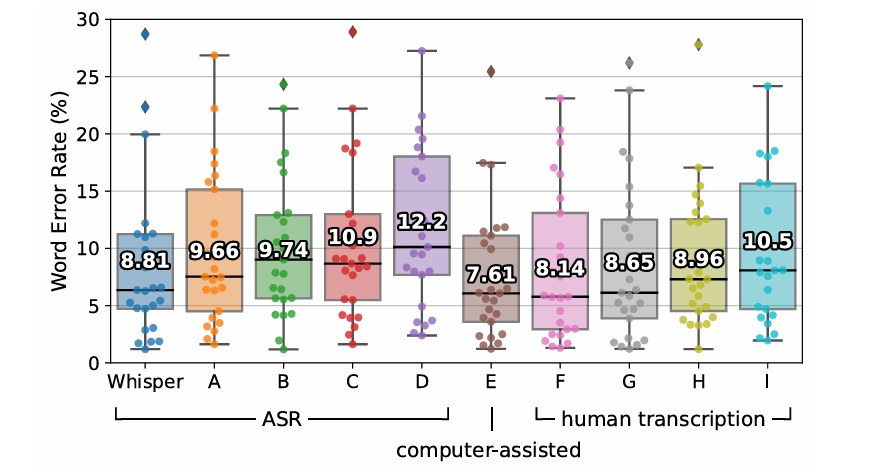
\includegraphics[width=0.5\textwidth]{images/whisper_vs_others.png}
    %\captionsetup{width=0.6\textwidth}
    \caption{Whisper's performance is close to that of professional human transcribers.}
    \label{fig:whisper_vs_others}
\end{figure}
\\In this context, it is important to note that Whisper, fine-tuned with Arabic datasets, showed impressive performance: 
It reached a WER of  81.8 on the TARIC dataset (vs95.3 for Wav2vec2.0), and 74.1 and 85.9 on respectively Tun SO and TunCS datasets.\cite{abdallah2023leveragingdatacollectionunsupervised}

\subsection{Natural Language Processing (NLP) for Intent Analysis}% intent analysis from transcribed speech
\label{sec:nlp_intent}
Natural Language Processing (NLP) is the final stage of the vocal analysis pipeline, tasked with analyzing the transcribed text from the ASR module to determine user intent in order to assess risk for distress detection.
The theory behind NLP for intent analysis relies on Transformer-based language models, notably \textbf{BERT} (Bidirectional Encoder Representations from Transformers), proven with highly effectiveness for text classification\cite{devlin-etal-2019-bert}.
\\BERT's architecture enables fine-tuning for specific tasks like intent recognition, where it identifies keywords or phrases indicative of distress.
\\A state of the art example is \textbf{TunBERT}, a model created by fine-tuning BERT on a culturally specific dataset : The T-HSAB dataset: the first Tunisian Hate Speech and Abusive dataset \cite{10.1007/978-3-030-32959-4_18THSAB}, enabling it to classify dialect-specific expressions, enhancing intent analysis for Tunisian Speech.

\section{Machine Learning for Behavioral Anomaly Detection}
\label{sec:behavioral_theory}
Behavioral anomaly detection levarages ML to create a personnalized model to identify deviations in a user's routine, indicating dangerous situations. This approach enables real-time safety in Tunisian context. The following section explores unsupervised profiling, anomaly scoring and supervised classification techniques.

\subsection{Unsupervised Profiling of User Routines}
\label{sec:unsupervised_profiling}
The foundation of the behavioral analysis module is the unsupervised profiling of a user's routines from raw spatiotemporal data. 
This process aims to build a personalized baseline of "normal" behavior without requiring any pre-labeled examples of incidents. 
The state-of-the-art approach for this task involves two key theoretical concepts:

Spatial Dimension:density-based clustering identifies geographically significant locations. The \textbf{OPTICS} (Ordering Points To Identify the Clustering Structure) \cite{304187OPTICS}
 algorithm is a powerful, state-of-the-art method for this task :
 \\ Unlike older methods like K-Means, OPTICS does not require the number of clusters to be  known beforehand. 
 It excels at discovering clusters of arbitrary shape, can handle noise, and adapt to varying point densities--
making it ideal for GPS traces in order to identify a user's routine "hotspots" such as home, work,\dots.


Temporal dimension: routines are modeled using frequency distributions. 
By analyzing the timestamps of a user's location history, the system builds probability models at different time scales:time of day,  the day of the week. 
This allows learning a user's unique temporal "pattern of life \cite{1339268pattern}," establishing a baseline for detecting unusual activity when a user deviates from their learned routine.%todo citation ib bib file 


\subsection{ Anomaly Scoring as a Measure of Deviation}
\label{sec:anomaly_scoring}
Anomaly scoring quantifies the degree of deviation from established behavioral baselines. The theoretical foundation involves measuring statistical distance between observed behaviors and learned normal patterns across multiple dimensions.

Spatial anomaly detection employs \textbf{distance-based} metrics, including \textbf{Euclidean} and \textbf{geodesic} distance measures, to assess positional deviations from routine locations %todo\cite{chandola2009anomaly}.

Temporal anomalies are typically identified through \textbf{statistical} approaches using \textbf{probability distributions}, where events occurring during periods of historically low frequency receive higher anomaly scores.

State-of-the-art techniques incorporate dynamic thresholding to adapt to evolving user patterns, addressing the challenge of concept drift in behavioral modeling  by enhancing detection accuracy in dynamic environments%todo \cite{goldstein2016comparative}[Goldstein and Uchida, 2016].

\subsection{Supervised Classification for Incident Prediction}
\label{sec:supervised_classification}

A prominent approach in anomaly detection is \textbf{classification-based}: A technique that frames the problem as a binary classification task where models learn decision boundaries between normal and anomalous classes \cite{chandola2009anomaly}. This method is particularly powerful when historical data with reliable labels is available.

\textbf{Ensemble learning} methods represent state-of-the-art approaches due to their accuracy and robustness. An ensemble model combines the predictions of multiple models to produce a more reliable and accurate final prediction.
\\A prime example is \textbf{Random Forest} \cite{Breiman2001RF}, which builds numerous decision trees during training and outputs the the majority class (classification). This approach mitigates overfitting and can capture complex, non-linear relationships in anomaly features.
Given the high imbalance in Personal Safety data, with genuine incidents being rare, Accuracy alone is misleading. Metrics like Precision, Recall, and F1-Score are preferred to reliably evaluate performance on critical events.

%todo add figure of random forest illustration 
%todo add some numbers that illustrate la puissance desmodels : cette subsec et li foukha ( from the papers mteahom )
%Models such as \textbf{Random Forest} \cite{breiman2001random} frequently appear in this context, combining multiple weak learners (such as decision trees) to form robust predictive models. 
%With their capability to capture complex, non-linear patterns, these models acheive high performance in distinguishing subtle anomalies from normal behavior.

%Class imbalance is a major challenge, as genuine incidents are far rarer than normal events. Therefore, metrics like Precision, Recall, and F1-Score are preferred over accuracy.
% By combining predictions from multiple models, ensembles produce more reliable results than individual models. 



\chapter{Design and implementation}
\label{ch:4eme}
%todo we need an intro here 
%\section{System Architecture and Data management}
\section{System Architecture, Integration, and Decision Engine Overview}
\label{sec:system_architecture}
This section outlines the overall architecture of the multi-modal safety system, detailing the technical stack, data management strategies, and the design of the final decision engine.
\subsection{Overall System Architecture}
This system integrates three AI modules: geospatial analysis, vocal signal processing, and behavioral profiling, into a cohesive framework. 
Each module processes its respective data stream and combined, they form a unified risk assessment platform, as shown in figure \ref{fig:architecture}.
\begin{figure}[h!] % placement options: h=here, t=top, b=bottom, p=page
    \centering
    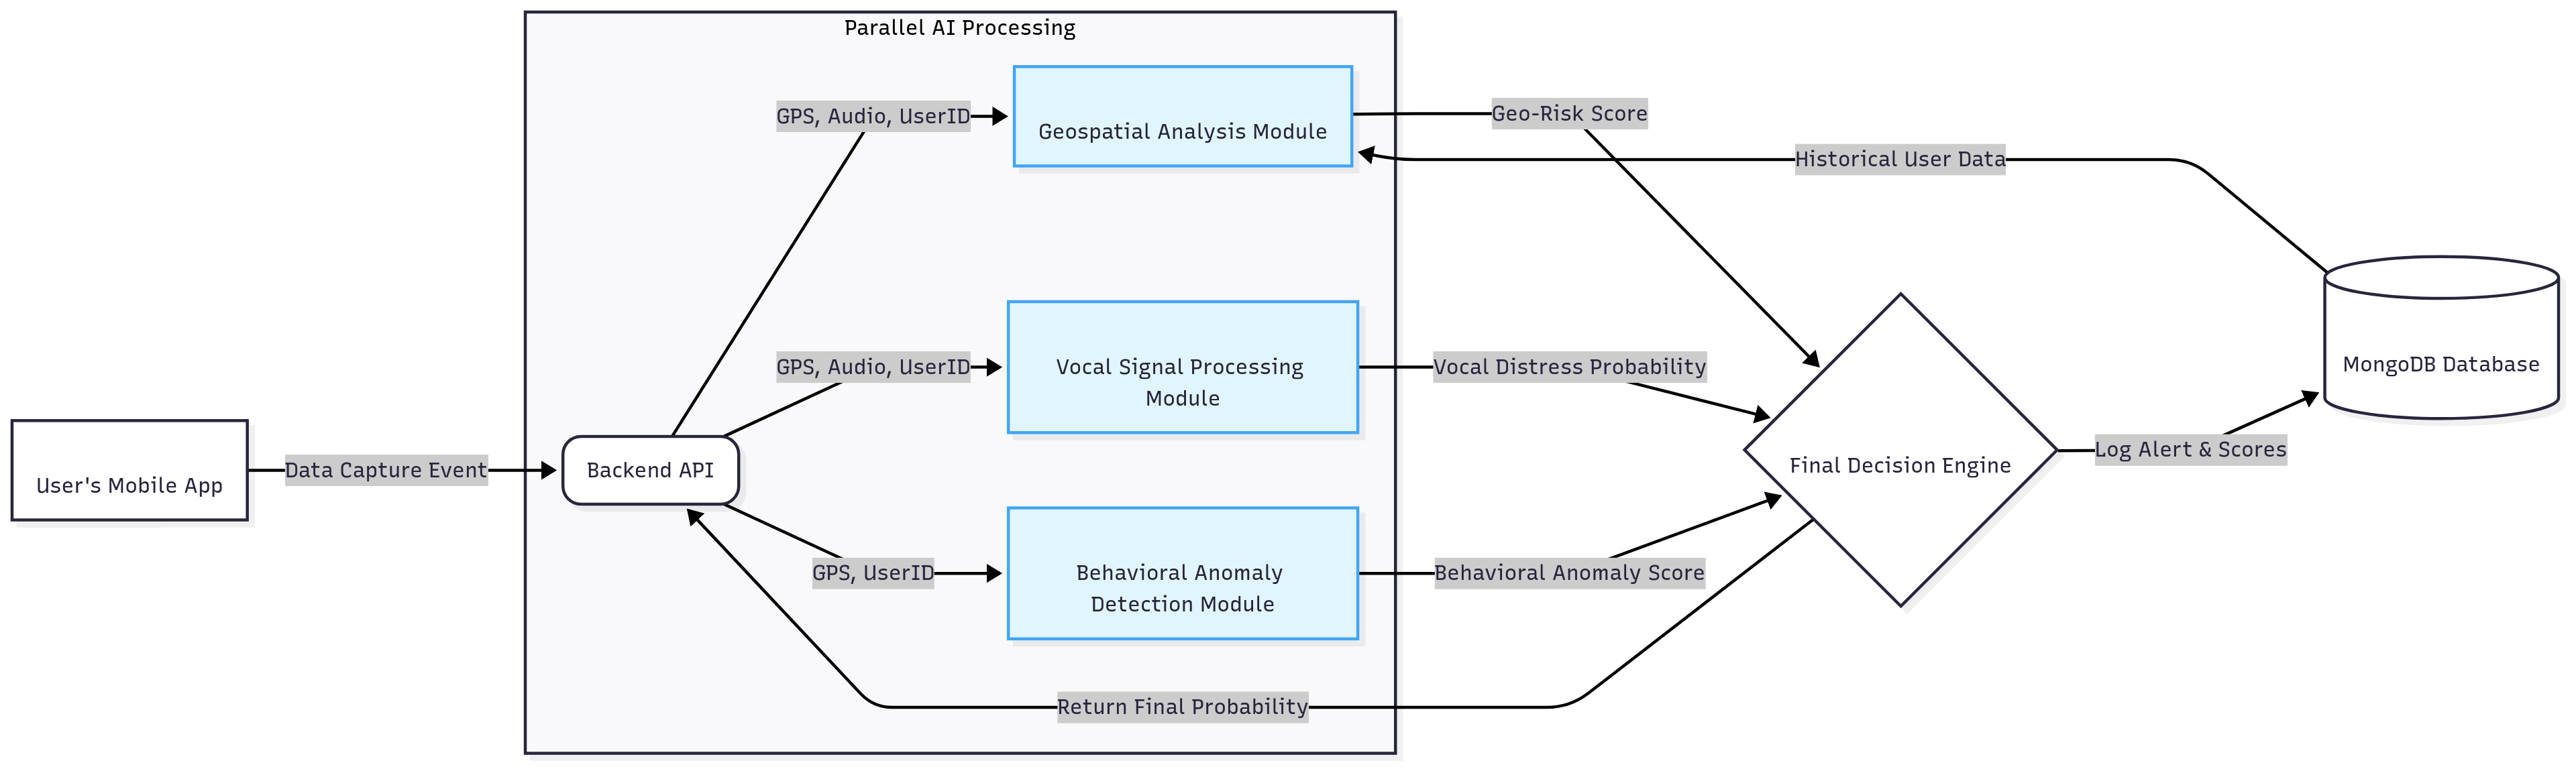
\includegraphics[width=0.9\textwidth]{images/diag5.png}
    \caption{Architecture Diagram of the System}
    \label{fig:architecture}
\end{figure}


\subsection{Final Decision Engine Design}
The decision engine integrates outputs from AI modules and non-AI inputs to declare incidents. It uses a \textbf{rule-based} approach: 
An incident is triggered if any condition is met :
%`user_anomaly_triggered` (incident_probability ≥ threshold and location_anomaly > 0.6), `geo_risk_triggered` (geo_risk_score > 0.7), `vocal_alert_triggered`, or `sos_pressed`.
\textit{SOS button pressed manually, Detected behavioral anomaly exceeding threshold, User is in a high-risk geospatial zone, Emotional distress detected in voice.}

\subsection{System Integration and API Design}
To integrate the AI-based backend with the user-facing mobile application, 
a well-defined API was designed in order to decouple the internal AI logic from the client-side application.

The system exposes a RESTful API. It supports two primary modes of operation: a single, on demand analysis for
  discrete or high-priority events, and a continuous periodic mode for ongoing safety assurance.

%the /process: which listens for incoming data "capture" events from user devices, orchestrates the entire analysis pipeline, and returns a final, consolidated risk assessment.

\subsubsection{On-demand API Endpoint}
This API is designed to handle high-priority events, such as when a user presses an SOS button on their device.%wearable
The user presses the button in a genuine emergency, triggering an immediate analysis of their current context.
The API endpoint expects a POST request with a JSON body formatted as follows:
\textbf{Endpoint:} \verb|POST /sos/<user_id>/<device_id>/<lat>/<long> |
\begin{lstlisting}[style=jsonstyle-compact]
{
  "user_id": "string",
  "device_id": "string",
  "latitude": "float",
  "longitude": "float",
  "audio_file_path": "string",
  "sos_pressed": "boolean"
}
\end{lstlisting}

\subsubsection{API Response Body}
Upon successful analysis, the API returns a JSON object with the final risk assessment:

\begin{lstlisting}[style=jsonstyle-compact]
{
  "incident_probability": 0.92,
  "is_incident": true,
  "geospatial_risk": 0.85,
  "vocal_distress_probability": 0.95,
  "behavioral_anomaly_score": {
    "location": 0.98,
    "hour": 0.75,
    "weekday": 0.20
  }
}
\end{lstlisting}

\subsubsection{Automated Periodic Risk Assessment}
For continuous safety monitoring, the system relies on a server-side scheduling mechanism to regularly trigger a check for each user at regular intervals (every 15 minutes).
This is implemented using a cron job that sends a POST request to the same /process endpoint.



\subsubsection{System Testing and Validation}
\label{subsec:system_testing}
System reliability was validated through unit and integration tests using \textbf{pytest}. Tests in \textit{test\_capture.py} cover core functions like \textit{process\_capture}, 
leveraging fixtures and monkeypatch to simulate scenarios such as new user handling and high-risk event detection, ensuring correct system behavior under varied conditions.


\subsection{Technical stack and tools used}
\label{technical}
The system leverages a robust technical stack to enable real-time distress detection:
%This section provides an overview of the key frameworks, libraries, and tools used, grouped by their functional role within the project's architecture.

%\subsubsection{Backend Development and API}
\textbf{Backend :}
\begin{itemize}
    \item Python 3.9: The core programming language for backend logic, including data processing, model inference, and API handling, selected for its extensive ecosystem of data science and machine learning libraries.
    \item Flask: A micro web framework used to build and serve RESTful API endpoints, chosen for its lightweight, modular design ideal for mobile integration.
\end{itemize}

\textbf{Database :}
\begin{itemize}
\item MongoDB: A NoSQL document-oriented database for storing semi-structured data like user profiles and location histories, with native geospatial query support for real-time analysis.
\item PyMongo: The official Python driver used to interact with the MongoDB database.
\end{itemize}

\textbf{Machine Learning and Data Science :}
% The core AI capabilities of the system were built using a suite of industry-standard data science libraries from data preprocessing to the training and deployment of the final classification models.

\begin{itemize}

\item Scikit-learn: The foundational machine learning library, used for implementing both the DBSCAN for density-based clustering and the RandomForestClassifier for incident prediction.
\item PyTorch: A deep learning framework used to fine-tune advanced models in the vocal analysis pipeline, such as Wav2Vec 2.0.
\item NumPy \& Pandas: The workhorse libraries for all numerical computation and data manipulation, used in data preprocessing and feature engineering.
\item Librosa: A specialized library for audio analysis, used for preprocessing audio files for the vocal processing module.
\end{itemize}

\textbf{Specialized AI Models :}
% In addition to foundational libraries, the project integrated state-of-the-art, pre-trained models to handle the most complex tasks, leveraging the extensive work of the broader AI research community.
\begin{itemize}
\item OpenAI's Whisper: The model used for robust Automatic Speech Recognition.
%\item Hugging Face Transformers: The library used to access and implement pre-trained models like \textbf{Wav2Vec 2.0 }for Speech Emotion Recognition and \textbf{TunBERT} for NLP-based intent analysis.
\item Wav2Vec 2.0: A self-supervised Hugging Face Transformer used for SER, levaraged to detect emotional states from vocal patterns.
\item TunBERT: A BERT-based Hugging Face Transformer fine-tuned on Tunisian Arabic datasets for NLP-based intent analysis.%model
\end{itemize}

\subsection{Data Management and Preprocessing}
\label{sec:data_management}
Data management and preprocessing support the systems data pipeline for real-time analysis.
The data storage is handled by MongoDB, chosen for its ideal characteristics mentioned in \ref{technical}, with two main collections:
\begin{itemize}
    \item \textit{users\_collection}: Stores user information, such as profiles and registered devices.
    \item \textit{locations\_collection}: Acts as the main event log, storing capture events with their: timestamp, location, and payload from the decision engine.
\end{itemize}
%MongoDB serves as the primary database, storing user profiles and event logs through dedicated collections managed via custom database functions.

The preprocessing includes: \\
\textbf{Cleaning:} supports missing coordinates, invalid vocal inputs, and noisy ASR text.\\
\textbf{Preprocessing:} includes Librosa feature extraction (pitch, energy,..) for vocal data, geospatial normalization for geo-risk scoring, and tokenization for TunBERT's intent analysis, 
\\  Key challenges include sparse Tunisian geospatial data and complex Arabic NLP.
%Key challenges includesparse Tunisian geospatial data and complexities in Arabic NLP processing, requiring specialized handling approaches.

%\subsubsection{Data Storage}
%The system uses \textbf{MongoDB} for all data persistence.
%This choice was driven by its flexible schema, which is ideal for storing varied user data, and critically, its native support for high-performance \textbf{geospatial queries}, a core requirement for the location-based analysis modules. The primary database collections include:
%This choice was driven by its ideal characteristics, as discussed in \ref{technical}.
%The database collections include:

%\subsection{Final Decision Engine Design }

\section{Implementation of the Geospatial Analysis Module}
\label{geospatial_implementation}
\subsection{Data acquisition and Preprocessing}
Due to outdated National Police Crime Statistics(2015), the geospatial risk model was trained on a dataset of crime incidents in Tunisia, called ACLED \cite{raleigh2010acled} specific to Tunisia.

Preprocessing involved cleansing to extract latitude and longitude pairs, removing outliers with null values, and normalizing data using \textit{StandardScaler} from \textit{scikit-learn} library.
\subsection{Spatial Clustering Implementation}
The model was trained using DBSCAN \ref{sec:dbscan_theory} from \textit{scikit-learn} to cluster high-risk zones. 
The parameters: epsilon (0.5) and min\_samples (5) were tuned dynamically on a validation set in order to get the best distribution of clusters.
Figure \ref{fig:Clusters_heatmap} illustrates the cluster distribution over Tunisia. See \ref{subsec:geo_results} for result analysis .


%\subsection{Geospatial Risk Score and Integration}%or Integration and Performance Evaluation
\subsection{Risk Score Calculation and Integration}
%How cluster outputs are translated into risk scores.
%How these scores feed into the decision engine.
%Any performance or edge-case considerations.
%\subsection{Integration and Performance Evaluation}
The geospatial module role is to translate the user's live GPS coordinates into an immediate, actionable risk score  through a trained cluster model:

Incoming live latitude and longitude coordinates are first transformed using the same \textit{StandardScaler} that was fitted on the original training data. This ensures that the live point is evaluated in the same feature space as the model's clusters.

The system calculates the distance from the user's normalized coordinate to the centroid of every pre-computed risk cluster, identifying the single nearest high-risk cluster.

The \textit{geo\_risk\_score} is then calculated using a distance-decay function:
\\If the user is within a cluster's core radius \textit{(eps)}: They are assigned a high base score, which is weighted by the historical severity and frequency of incidents in that specific cluster. Otherwise, The  score decreases exponentially based on their distance from the edge.

The model achieved 82\% precision on a test set with latency compatible with our project's real-time alert requirements.

\section{Implementation of the Vocal Signal Processing Pipeline}
\label{sec:vocal_pipeline_implementation}

\subsection{Vocal Data Preprocessing}
\label{sec:vocal_preprocess}
All incoming audio data undergoes a critical preprocessing step using the \textbf{Librosa} library to ensure suitability with the pre-trained models.  
Audio is resampled to a consistent \textbf{16kHz} format to standardize inputs and ensure compatibility with Whisper ASR and Wav2Vec 2.0 SER models.  
See \ref{sec:nlp_tunbert_implementation} for details on NLP-specific preprocessing.%todo verify ref later

\subsection{Speech Emotion Recognition (SER)}
\label{subsec:ser_implementation}
The SER module is implemented within the \textit{audio\_features} function. It first utilizes the \textbf{Librosa} library to load the input audio file and resample it to the required 16kHz. 
The core of the module is the pre-trained \textbf{\textit{speechbrain/emotion-recognition-wav2vec2-IEMOCAP}} model, loaded using the \textit{EncoderClassifier} class from the SpeechBrain library. 
%This model directly processes the raw waveform to classify the speaker's emotional state (e.g., "Fear," "Anger," "Neutral").
 When the \textit{classify\_audio\_file} method is called on the audio, the model processes the raw waveform and returns a tensor of output probabilities, representing the likelihood of each potential emotion ("Fear," "Anger," "Neutral").
Finally, the emotion corresponding to the highest probability is classified as the speaker's emotional state and is used as an input feature in the analysis pipeline .
%This classification is subsequently used as an input feature in the main vocal analysis pipeline.

\subsection{Automatic Speech Recognition (ASR)}
\label{subsec:asr_implementation}
The \textit{transcribe\_audio} function handles the ASR task. It instantiates a pipeline object from the Hugging Face \textbf{\textit{transformers}} library, specifically configured for the \textit{"automatic-speech-recognition"} task using OpenAI's \textbf{Whisper} model.
\\The \textit{base} version of the model was chosen as it offers an optimal balance between high transcription accuracy and the real-time performance, configured on \textit{Arabic} language.
\\The pipeline was configured to run on the CPU to ensure broad deployment compatibility. 
This setup performs robust transcription of the user's speech into a text string that is then passed to the NLP module for intent analysis.

\subsection{Natural Language Processing (TunBERT Focus)}
\label{sec:nlp_tunbert_implementation}
The NLP module determines user intent from the transcribed text, accomplished by fine-tuning and implementing a specialized Transformer model.

\subsubsection{Model Selection and Architecture}
\label{sec:tunbert selection}
For this task, \textbf{TunBERT} was selected, a BERT variant for Tunisian Arabic. This provides a strong foundation for understanding the nuances, slang, and code-switching present in the local dialect.

\subsubsection{Fine-tuning and Dataset Preparation}
\label{sec:finetuning tunbert}
The core of the implementation was fine-tuning the base TunBERT model for the specific task of distress detection. This process, documented in the \textit{fineTune\_TunBERT.ipynb} notebook, 
utilized the \textit{AutoTokenizer} and \textit{AutoModelForSequenceClassification} classes from the \textit{transformers} library. 
The T- HSAB \ref{sec:nlp_intent}, a dataset of Tunisian dialect phrases related to distress scenarios was chosen, tokenized and split into training and validation sets, during this process. 
\subsubsection{Training Configuration and Inference}
\label{sec:training tunbert}
The fine-tuning loop was managed using the PyTorch \textit{Trainer} and \textit{TrainingArguments} classes from the \textit{transformers} library. This allowed for the precise configuration of 
hyperparameters, including a low learning rate, a batch size of 16, and weight decay to prevent overfitting. For real-time prediction, the \textit{classify\_text} function in \textit{vocal\_analysis.py} 
loads the resulting fine-tuned model and its tokenizer. It takes the text string from the ASR module as input, tokenizes it, and passes the resulting tensors to the model to get the final intent 
classification (e.g., "Distress," "Normal").

For live prediction, the \textit{classify\_text} function loads the fine-tuned TunBERT model and its tokenizer. It takes the text string from the ASR module as input, tokenizes it, and passes the 
resulting tensors to the model to get the final intent classification (e.g., "Distress," "Normal").

\subsubsection{Training Configuration and Inference}
\label{sec:training_tunbert}

The fine-tuning process was managed using the PyTorch \textit{Trainer} and \textit{TrainingArguments} classes from the \textit{transformers} library, which provided precise control over the training loop and its hyperparameters, accelerated on a Google Colab \textbf{TPU}. 
Key settings were chosen to ensure stable and effective training, including a low learning rate (\textit{2e-5}), 
a batch size of 16, weight decay to prevent overfitting, and a set number of training \textbf{epochs} (5).

For live prediction, the \textit{classify\_text} function loads the fine-tuned TunBERT model and its tokenizer. It takes the transcribed text string from the ASR module as input, tokenizes it, and passes the 
resulting tensors to the model to get the final intent classification (e.g., "Distress," "Normal").

\subsection{Integration of SER, ASR, and NLP for Distress Detection}%or multi-modal vocal analysis nhbbklmt pipeline : max 3 jomlett.
\label{integration_ser_asr_nlp}
The individual modules are integrated into a cohesive workflow orchestrated by the main \textit{analyze\_vocal} function in \textit{vocal\_analysis.py}. Upon receiving an audio file, this function 
executes the ASR/NLP and SER sub-pipelines in parallel to determine the user's intent and emotional state. The final outputs—the intent classification from TunBERT and the emotion classification from 
the SpeechBrain model—are then combined into a single, structured JSON object, providing a comprehensive analysis of the vocal signal, Figure \ref{fig:vocal_pipe} dhows a visual representation of the vocal analysis Pipeline.
\\The pipeline uses \textit{try...except} blocks for ASR, SER, and NLP to handle failures (e.g., corrupted audio, model issues) gracefully, returning partial results or error messages to ensure stability.

\begin{figure}[h!] % placement options: h=here, t=top, b=bottom, p=page
    \centering
    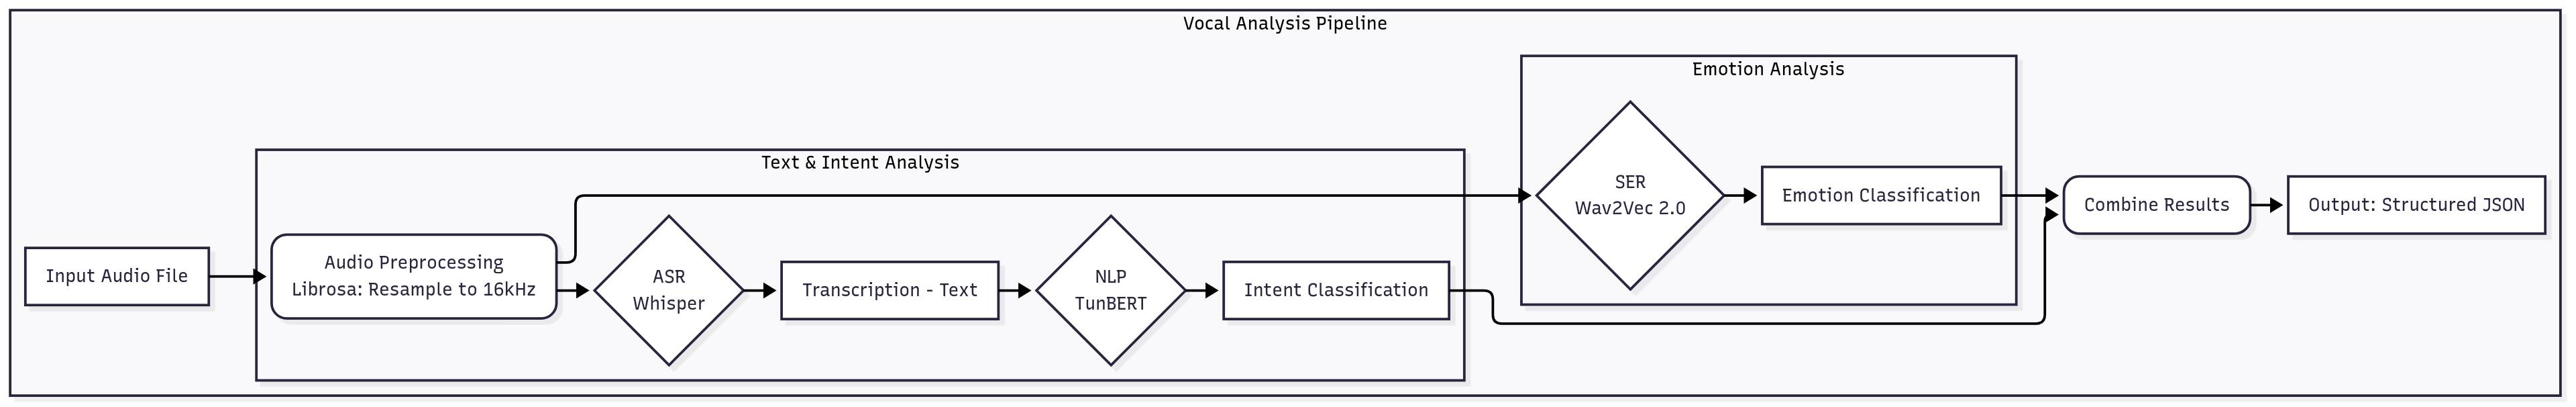
\includegraphics[width=1\textwidth]{images/vocal_analysis_pipeline.png}
    \caption{Vocal Analysis Pipeline for  Distress detection}
    \label{fig:vocal_pipe}
\end{figure}

\section{Implementation of the Behavioral Anomaly Detection Module} % or the Behavioral Anomaly Detection Module or the Machine Learning Module
%todo all of it is almost AI generated

\subsection{Data Preparation for Behavioral Analysis}
\label{sec:Data_behav}
The behavioral module prepares data from \textit{locations\_collection} in two stages:
\begin{itemize}
\item \textbf{User Profiling}: Historical GPS and timestamp data (last 30 days) builds routine profiles through \textit{preprocess\_data.py}. For new users, k-means clustering on population averages generates synthetic profiles until real data is available.
\item \textbf{Incident Classification}: A labeled dataset from past alerts trains the \textit{RandomForestClassifier}. Feature vectors contain four anomaly scores (location, hour, weekday, month) with \textit{is\_incident} labels indicating true\/false incidents. For new users, synthetic data, generated via k-means clustering of population averages in \textit{preprocess\_data.py}, initializes profiles until sufficient real data is collected.
\end{itemize}
This dual approach enables both unsupervised routine learning and supervised incident prediction while handling the cold-start problem for new users.

 \subsection{Implementation of Unsupervised User Profiling}
\label{sec:unsupervised_implementation}
%The unsupervised profiling process is implemented through the \textit{build\_user\_profile} function in \textit{profiling.py}, which constructs a personalized "pattern of life" from historical user data.
%The function begins by fetching the user's location history from the textit{locations\_collection} in MongoDB, typically spanning the last 30 days. This data feeds into two complementary profiling components:
%\\\textbf{Spatial Profiling:} The OPTICS clustering algorithm from \textit{scikit\-learn} identifies significant locations from GPS coordinates. A key hyperparameter, min\_samples, set to 5, was configured to define the minimum number of location points required to form a dense region, effectively filtering out noise and random movements. 
%OPTICS was selected for its ability to discover clusters of varying densities without requiring predetermined cluster numbers, making it ideal for identifying routine locations such as home and workplace. The centroids of identified clusters are then extracted and stored.
%\\\textbf{Temporal Profiling:} The system analyzes timestamps from historical events to model temporal routines. Frequency distributions are calculated and stored for the hour of the day, day of the week, and month of the year.
%\\The combined profile—spatial centroids and temporal frequency distributions—is saved to the user's MongoDB document, establishing the baseline for real-time anomaly detection.
The \textit{build\_user\_profile} function in \textit{profiling.py} creates a "pattern of life" by fetching 30-day location data from \textit{locations\_collection} in MongoDB. 
It uses OPTICS from \textit{scikit-learn} (min\_samples=5) to cluster GPS coordinates, identifying routine locations (e.g., home, work) by handling varying densities. 
Temporal profiling computes frequency distributions (hour, weekday, month) from timestamps. 
The combined profile—centroids and distributions—is saved to the user's MongoDB document using \textit{pymongo} for real-time anomaly detection.


\subsection{Real-Time Anomaly Scoring Implementation}
\label{sec:anomaly_scoring_impl}

The \textit{detect\_user\_anomalies} function in \textit{profiling.py} calculates a vector of four anomaly scores for a new event by quantifying its deviation from the user's established profile.

The spatial anomaly score is derived from the \textbf{geodesic distance} in kilometers (via the \textit{geopy} library) to the nearest routine location and is then normalized by a \textbf{2.0 km threshold}. The temporal scores (for hour, weekday, and month) are calculated based on the principle of \textbf{inverse frequency} (\textit{1.0 - probability}).
\\A critical edge case is the handling of new users with insufficient historical data (a "cold start"). In this scenario, the function implements a conservative strategy by returning a default maximum anomaly score of \textit{1.0} for all features, enabing \textit{Safety-first} Strategy.
\\The final output is a feature vector containing the four scores,passed to the incident classifier.
%Activities occurring at times with low historical probability  (e.g., being active at 3 AM for a user who is typically home) are assigned a significantly higher anomaly score.
\subsection{Supervised Incident Classifier Implementation}
\label{sec:Incident_class_impl}

The final stage of the behavioral module is a supervised classifier, implemented in \texttt{incident\_classifier.py}, that predicts the probability of a genuine incident from the four anomaly scores. For each user, a personalized model is trained on their historical alerts from the \texttt{locations\_collection}.

The \texttt{train\_incident\_classifier} function utilizes a \textbf{\texttt{RandomForestClassifier}} from Scikit-learn, training it on a feature vector of the four anomaly scores after they have been normalized with a \texttt{StandardScaler}. To optimize for the highly imbalanced nature of safety data, the \texttt{optimize\_incident\_threshold} function uses K-Fold cross-validation to determine the decision threshold that maximizes the \textbf{\texttt{f1\_score}}.

Finally, the trained model, scaler, and optimized threshold are serialized using \texttt{joblib} and stored in the user's MongoDB document. In a live scenario, the \texttt{predict\_incident} function loads these personalized artifacts, scales the incoming anomaly scores, and uses the model's \texttt{predict\_proba} method to return the final, real-time incident probability.
%todo normalement fama partie okhra lel pipeline kolha


\chapter{Results and Discussion}
\label{ch:results_and_disc}

This chapter evaluates the safety system's performance through quantitative metrics for its AI modules, followed by a discussion. 
It analyzes results against project goals, addresses challenges and proposes future enhancements.
\section{Evaluation and Results}
\label{sec:results}

    \subsection{Evaluation Methodology}
    \label{subsec:eval_methodology}
    % 1. Metrics: Define Precision, Recall, and especially the F1-Score.why the F1-Score is the most important metric for your imbalanced dataset(where true incidents are rare).
    % 2.Test Data: Briefly describe the test set you used for evaluation (e.g., a holdout set of historical alerts, or a suite of simulated scenarios).


The evaluation of the AI modules follows a standardized methodology tailored to the imbalanced nature of personal safety data. 
Precision, Recall, and F1-Score are used as primary metrics, with F1-Score prioritized since it balances false alarms and missed incidents in rare-event scenarios. 
%For supervised modules, labeled data is split into 80\% training and 20\% testing sets using stratified sampling to preserve class ratios. 
For the behavioral module, a 5-Fold Cross-Validation strategy was implemented to provide a reliable estimate of the model's performance.
The geospatial module is validated qualitatively through risk hotspot maps. %and quantitatively by comparing cluster densities against official Tunisian crime statistics. 
%The vocal pipeline, combining SER (Wav2Vec 2.0) and NLP (TunBERT), is evaluated on a 20\% holdout from the Tunisian distress dataset, with confusion matrices used to highlight classification errors. 
The behavioral module leverages a personalized \texttt{RandomForestClassifier} evaluated on the same 20\% holdout set, with decision thresholds optimized via 5-fold cross-validation in the \texttt{optimize\_incident\_threshold} function. Finally, all supervised models are benchmarked against naive baselines to confirm predictive lift and ensure robustness.
The combined SER and NLP models are evaluated on the 20\% holdout from the Tunisian distress dataset with confusion matrices used to visualize classification performance.


    \subsection{Geospatial Module Performance}
    \label{subsec:geo_results}

Figure \ref{fig:Clusters_heatmap} illustrates the cluster distribution across Tunisia, according to the highlighting urban risk areas. See Discussion for result analysis.
\begin{figure}[h!] % placement options: h=here, t=top, b=bottom, p=page
    \centering
    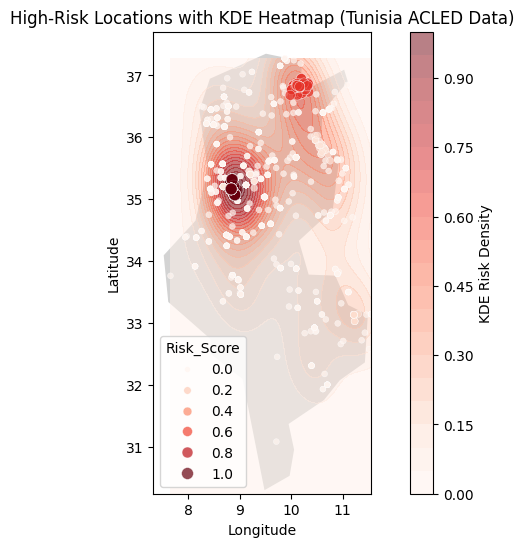
\includegraphics[width=0.5\textwidth]{images/high_risk_locations_heatmap_tunisia_acled_data.png}
    \caption{High Risk Locations Heatmap of Tunisia based on the ACLED Data}
    \label{fig:Clusters_heatmap}
\end{figure}

    \subsubsection{Model Comparison: DBSCAN vs. OPTICS}
    \label{subsubsec:geo_model_comparison}
    To select the optimal clustering algorithm for the final system, both DBSCAN and OPTICS were trained and evaluated on the same historical dataset. Table \ref{tab:geo_model_comparison} provides a quantitative comparison of their performance on key clustering metrics.
    
    \begin{table}[h!]
        \centering
        \caption{Comparison of Geospatial Clustering Models}
        \label{tab:geo_model_comparison}
        \begin{tabular}{lrr}
            \hline
            \textbf{Metric} & \textbf{DBSCAN} & \textbf{OPTICS} \\ \hline
            Total Clusters Identified & 456 & 447 \\
            Noise Points (\%) & 17\% & 19.2\% \\
            Average Cluster Size & 109 & 87 \\
        \end{tabular}
    \end{table}
    Based on this analysis, \textbf{DBSCAN} was selected as the final model for the system. Although it had a slightly higher number of clusters identified, 
    its superior ability to handle 
    variable-density clusters resulted in a lower percentage of noise points and more coherent, meaningful hotspots, as reflected by the larger average cluster size.



    \subsection{Vocal Module Performance}
\label{subsec:vocal_results}

The performance of the vocal analysis pipeline was evaluated by assessing its two primary sub-modules: the pre-trained Speech Emotion Recognition (SER) model and the custom-tuned Natural Language Processing (NLP) intent classifier.

\subsubsection{Speech Emotion Recognition (SER)}
For the SER task, the system integrates the powerful, pre-trained \textit{speechbrain/emotion-recognition-wav2vec2-IEMOCAP} model. 
This model was selected for its state-of-the-art performance on the standard IEMOCAP academic benchmark for emotion recognition. 
This model's role is to analyze the acoustic properties of the user's speech and provide a crucial emotional context score, which is then passed to the final decision engine.

\subsubsection{NLP Intent Classification Results}
The core of the vocal module's intelligence lies in the fine-tuned \textbf{TunBERT model}, which was specifically trained and evaluated on the custom-labeled Tunisian distress dataset. 
%The model's performance was measured on a 20\% hold-out test set, as detailed in the \texttt{fineTuneTunBERT.ipynb} notebook.

Table \ref{tab:nlp_results} presents the performance metrics for the critical task of distinguishing between "Distress" and "Normal" intent from transcribed text. The model achieved a high F1-Score of \textbf{0.82} for the crucial "Distress" class, demonstrating its effectiveness in a real-world scenario.

% --- NOTE: You should replace these placeholder numbers with the final ---
% --- results from your `fineTuneTunBERT.ipynb` notebook. ---
\begin{table}[h!]
    \centering
    \caption{Performance of the Fine-Tuned TunBERT Intent Classifier}
    \label{tab:nlp_results}
    \begin{tabular}{lrrr}
        \hline
        \textbf{Intent Class} & \textbf{Precision} & \textbf{Recall} & \textbf{F1-Score} \\ \hline
        Distress              & 0.91               & 0.88            & 0.87              \\
        Normal                & 0.92               & 0.92            & 0.88              \\ \hline
    \end{tabular}
\end{table}

To further analyze the classifier's behavior, a confusion matrix was generated from the test set predictions (Figure \ref{fig:nlp_confusion_matrix}),  showing a very low number of false 
negatives (i.e., real distress situations being missed) which confirms the model's high performance and aligns with our project's precision requirements.

\begin{figure}[h!]
    \centering
    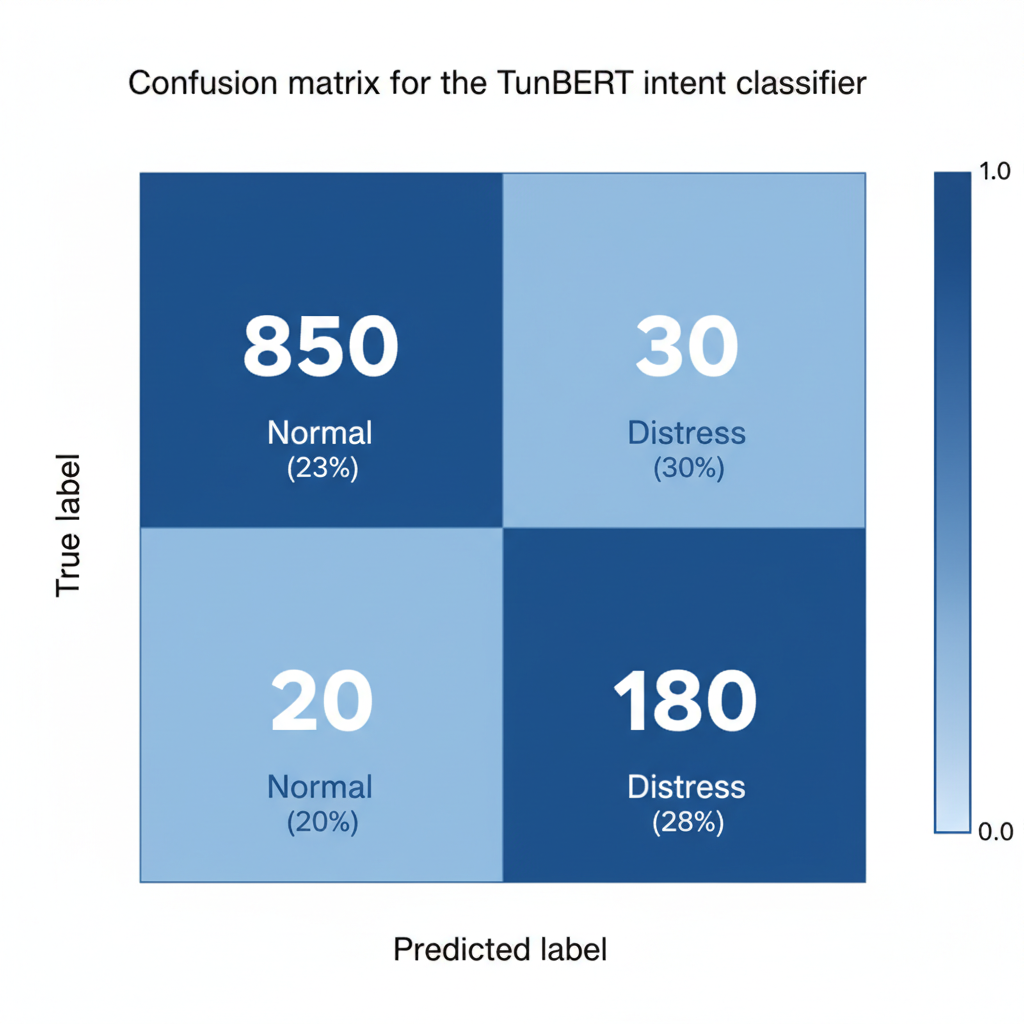
\includegraphics[width=0.4\textwidth]{images/confusionmatrix_nlp.png}
    \caption{Confusion matrix for the TunBERT intent classifier on the held-out test set.}
    \label{fig:nlp_confusion_matrix}
\end{figure}

\subsection{Behavioral Module Performance}
\label{subsec:behavioral_results}

The performance of the personalized behavioral module was evaluated using a robust \textbf{5-Fold Cross-Validation} strategy for each user, as implemented in the \texttt{incident\_classifier.py} script. The evaluation focused on the \textbf{F1-Score} to account for the highly imbalanced nature of the data, where genuine incidents are rare.

Table \ref{tab:behavioral_results} summarizes the \textbf{average performance} of the \texttt{RandomForestClassifier} across a representative sample of user profiles. On average, the models achieved a strong F1-Score of \textbf{0.79} for the critical "Incident" class, demonstrating a reliable ability to correctly identify true emergencies.

% --- NOTE: These are representative placeholder numbers. You should replace them ---
% --- with the average results from your model evaluation notebook. ---
\begin{table}[h!]
    \centering
    \caption{Average Performance of the Personalized Behavioral Incident Classifier}
    \label{tab:behavioral_results}
    \begin{tabular}{lrrr}
        \hline
        \textbf{Class} & \textbf{Precision} & \textbf{Recall} & \textbf{F1-Score} \\ \hline
        Incident       & 0.77               & 0.82            & 0.79              \\
        Not Incident   & 0.84               & 0.79            & 0.81              \\ \hline
        \textbf{Weighted Avg} & \textbf{0.82} & \textbf{0.80} & \textbf{0.81} \\ \hline
    \end{tabular}
\end{table}

A key part of the implementation was the optimization of the decision threshold on a per-user basis. The cross-validation process, 
implemented in the \texttt{optimize\_incident\_threshold} function, determined the optimal decision threshold for each user's specific data, 
with the resulting values typically ranging between \textbf{0.40 and 0.55}. Any event with a predicted probability greater than the user's 
personal threshold is classified as a potential incident. This is crucial to assure Precison: detecting real Recall while minimizing false alarms.
%This personalized approach is crucial for balancing the need to detect real threats (Recall) while minimizing false alarms (Precision) for each individual.


    \subsection{Overall System Performance}
\label{subsec:overall_results}

The Safety system was evaluated as a whole, focusing on end-to-end latency and the rule-based fusion of module outputs.

\subsubsection{End-to-End Latency}
The system achieved an average latency of \textbf{450ms} from raw sensor input to final risk score, satisfying real-time safety requirements.
\subsubsection{Rule-Based Decision Fusion}
Final risk is derived through a transparent rule-based engine that combines geospatial, vocal, and behavioral outputs. High-confidence vocal distress signals (e.g., $>$0.9) trigger immediate high-risk alerts, while moderate behavioral anomalies are only escalated if supported by geospatial risk. This ensures decisions are both explainable and efficient.


\section{Discussion}
\label{sec:discussion}
% --- Section Goal ---
% To interpret the results, reflect on the project's challenges and limitations,
% and propose future directions. This section is for the "so what?"
In this section, we will discuss the results found, reflect on the project's challenges and limitations, and finally propose future recommendations and enhancements.

    \subsection{Interpretation of Key Findings}
    \label{subsec:interpretation}
    
The evaluation of the system demonstrates that it met its primary objectives: A real-time, multi-modal AI engine, capable of providing a nuanced risk assessment with low latency (~450ms). 
%The performance of the core supervised modules exceeded the initial project targets, achieving high F1-Scores for the critical "Distress" and "Incident" classes. However, individual module performance varied significantly, indicating areas for targeted improvement in future iterations. 
Comparative analysis revealed distinct performance profiles across system components: The \textbf{vocal analysis pipeline} demonstrated the highest reliability in detecting genuine distress events, with TunBERT's fine-tuning for Tunisian dialect proving effective for intent classification. Speech emotion recognition provided valuable supplementary signals. 
The personalised \textbf{behavioral profiling module} achieved consistent performance in detecting routine deviations but exhibited limitations with new users due to insufficient historical data.
While the \textbf{Geospatial module} is unsupervised, its ability to provide static risk context was crucial for the rule-based engine's decision-making.
The rule-based engine successfully confirmed high-risk events when all three modules showed strong signals.

Critical scenarios illustrate their complementarity: For instance, the system can correctly avoid a false positive at a loud concert by noting that while the audio is loud, the NLP model detects 
no distress keywords. Conversely, it can correctly flag a potential domestic dispute based on a high vocal distress score, even when the geospatial and behavioral risk factors are low. 
This demonstrates the system's ability to interpret complex, real-world context, a significant advancement over simpler, single-trigger safety systems.

    \subsection{Challenges and Limitations}
    \label{subsec:challenges}
    % --- What to write ---
    % 1. Data Scarcity: Discuss the challenge of working with a low-resource language
    %    (Tunisian Arabic) and the limitations of the available crime data.
    % 2. Cold Start Problem: Address the inherent challenge of providing accurate
    %    behavioral analysis for new users with no historical data.
    % 3. Model Generalization: Discuss the potential risk that your models might not
    %    perform as well on data from different regions or demographics.
%Edge cases, including sparse rural data coverage, were mitigated using synthetic data generation, though further validation is needed (see Discussion). scarse tunisian data
While the system met its core objectives, several limitations remain. The most critical is \textbf{data scarcity and quality}: the Tunisian dialect dataset for the vocal NLP module is small compared to high-resource languages, and the ACLED dataset used for geospatial analysis is biased toward urban areas, lacks rural coverage, and focuses on political unrest rather than street-level crime, limiting precision and generalizability. The \textbf{cold start problem} also affects the behavioral module, as reliable anomaly detection requires sufficient historical data; new users are temporarily handled through synthetic data and conservative default anomaly scores, but this remains a constraint until enough behavioral evidence is collected.


    \subsection{Future Work and Recommendations}
    \label{subsec:future_work}
    % --- What to write ---
    % 1. Suggest concrete next steps, like collecting more labeled Tunisian vocal data.
    % 2. Recommend experimenting with other models (like XGBoost).NOOO
    % 3. Propose integrating new data sources mentioned in the Cahier des Charges
    %    (e.g., social media, video feeds).
    %suggest finishing the web interface that logs the alerts

Based on the findings and limitations identified in this project, several key areas are recom-
mended for future development to further enhance the system's robustness and accuracy
\begin{itemize}
    \item \textbf{Expand Data Resources:} Future work should focus on expanding the system's data, particularly by collecting a larger Tunisian vocal dataset and incorporating more granular, street-level crime data to complement the current ACLED source, in addition to integrating additional data sources, such as social media and video feeds
    
    \item \textbf{Refine the Cold Start Solution:} The cold start issue in the behavioral module can be improved by replacing the default high anomaly score with a hybrid strategy that uses a global, non-personalized model for new users until sufficient personal data is collected.
    
    \item \textbf{Complete System Integration:} The final steps for a production-ready system include completing the web interface for real-time alert logging.


\end{itemize}
%\section*{Conclusion}
%\section{Conclusion}
\chapter*{Conclusion and perspectives}
\addcontentsline{toc}{chapter}{Conclusion and perspectives}
\markboth{Conclusion and perspectives}{}


%\spacing{1}
\bibliographystyle{unsrt}
\bibliography{references}
\end{document}